Let $N$ be a positive integer. A collection of $4N^2$ unit tiles with two segments drawn on them as shown is assembled into a $2N\times2N$ board. Tiles can be rotated.
\begin{center}
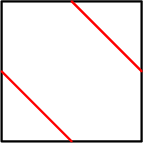
\includegraphics[width = 14.4mm]{img/fig0.png}
\end{center}
The  segments  on  the  tiles  define  paths  on  the  board. Determine  the  least  possible  number  and  the largest possible number of such paths.

\textit{For example, there are $9$ paths on the $4 \times 4$ board shown below.}
\begin{center}
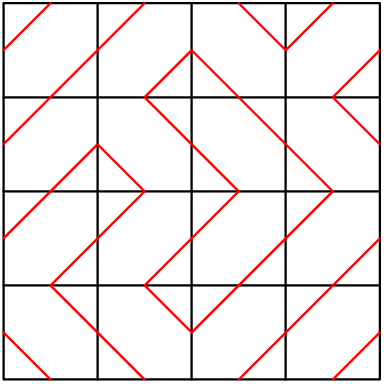
\includegraphics[width = 38.400000000000006mm]{img/fig1.png}
\end{center}
